\documentclass[12pt,oneside,a4paper]{book} % This style for A4 format.

\input{./AuxFiles/Packages}

%%%%%%%%%%%%%%%%%%%%%%%%%%%%%%%%%%%%%%%%%%%%%%%%%%%%%%%%%%%%%%%%
%% Document settings
\title{An Integrated Edge-AI Emergency Healthcare Platform for Elderly Fall Prediction Using Wearable Sensors and Real-Time Ambulance Coordination}
\subCode{XX367P}
% Note: While using the template for IDP, the \Department cmd is not used (discarded automatically) in IDP. The Certificate page uses \guideDeptA[]{} cmd in IDP.
\Department[CSE]{Computer Science and Engineering}
\academicYear{Even 2025-26}

% Paragraph formatting
\setlength{\parindent}{0pt}
\setlength{\parskip}{0.5em}

%%%%%%%%%%%%%%%%%%%%%%%%%%%%%%%%%%%%%%%%%%%%%%%%%%%%%%%%%%%%%%%%
%% Report Type:
%%%%%%%%%%%%%%%%%% For Plagiarism Check %%%%%%%%%%%%%%%%%%%%%%%
%% Uncomment \EnPlagReport line, before plagiarism check to remove Certificate, Declaration, Acknowledgement and TOC pages.
%\EnPlagReport

%%%%%%%%%%%%%%%%%%%%%% IDP report %%%%%%%%%%%%%%%%%%%%%%%%%%%%%
%% Uncomment \IDPProject line, if the report is for IDP project.
\IDPProject

%%%%%%%%%%%%%%%%%%% For PG program %%%%%%%%%%%%%%%%%%%
%% Uncomment \pgProgram command and define appropriate values for \MastersIn{} and \pgProgramName{}

%\pgProgram%
\MastersIn[M.Tech]{Master of Technology}
\pgProgramName{VLSI Design \& Embedded Systems}

%%%%%%%%%%%%%%%%%%%%%%%%%%%%%%%%%%%%%%%%%%%%%%%%%%%%%%%%%%%%%%%%
%% Student Details%%%
\stuNameA{M P Preetham}
\stuUSNA{1RV23CS122}
\stuNameB{Gagan B C}
\stuUSNB{1RV23CS090}
\stuNameC{Amaresh Malgi}
\stuUSNC{1RV24EC015}
\stuNameD{Gokul P}
\stuUSND{1RV24EC403}
%%\stuNameE{}
%%\stuUSNE{}
%%\stuNameF{}
%%\stuUSNF{}

%%%%%%%%%%%%%%%%%%%%%%%%%%%%%%%%%%%%%%%%%%%%%%%%%%%%%%%%%%%%%%%%
%% Guide Related commands
%% Internal Guide %%
% Have to give both short form and long of Department Name
\guideNameA{Dr. Tabitha Janumala}
\guideDesignationA{Assistant Professor}
\guideDeptA[EIE]{Electronics and Instrumentation Engineering}
\guideOrgA{RV College of Engineering}


%%%%%%%%%%%%%%%%%%%%%%%%%%%%%%%%%%%%%%%%%%%%%%%%%%%%%%%%%%%%%%%%
%% Esteem members related commands
%% Pannel Members %%
\panelMemberNameA{Dr. Kariyappa}
\panelMemberDesigA{Professor}
\panelMemberDeptA[CSE]{Computer Science and Engineering}
\panelMemberNameB{Prof. P N Jayanthi}
\panelMemberDesigB{Assistant Professor}
\panelMemberDeptB[CSE]{Computer Science and Engineering}

% Added Ver 3.6 & 3.9
%% Project co-ordinators (for Internal RVCE) 
\projectCoOrdNameA{Dr. Chetana G}
\projectCoOrdDesigA{Assistant Professor}
\projectCoOrdDeptA[CSE]{Computer Science and Engineering}

%%%%%%%%%%%%%%%%% Esteemed Members %%%%%%%%%%%%%%%%%%
\HOD{Dr. Ravish Aradhya}
\Principal{Dr. K. N. Subramanya}
% For IDP only
\DeanAcademics{Dr. M.V. Renukadevi}
\VicePrincipal{Dr. Geetha K S}
%%%%%%%%%%%%%%%%%%%%%%%%%%%%%%%%%%%%%%%%%%%%%%%%%%%%%%%%%%%%%%%%
%%%%%%%%%%%%%%%%%%%%%  QRL %%%%%%%%%%%%%%%%%%%%%%%%%%
\QRurl{}
%\QRurl{https://drive.google.com/open?id=1jm-POmuq-ZZ1tT5m-xAdCDRnwvLZH8q-}

%%%%%%%%%%%%%%%%%%Draft report%%%%%%%%%%%%%%%%%%
%\DraftCopy %Not yet implemented, if anyone interested, do contact me at pnarashimaraja@rvce.edu.in (or) narashimaraja@gmail.com
%%%%%%%%%%%%%%%%%%%%%%%%%%%%%%%%%%%%%%%%%%%%%%

%%%%%%%%%%%%%%%%%% Glossaries & Acronyms %%%%%%%%%%%%%%%%%%
\newglossary[sym]{symbolList}{sym1}{sym2}{List of Symbols}
\makeglossaries
% Acronyms
\loadglsentries{./AuxFiles/Glossaries}
\renewcommand{\glspostdescription}{}% To remove dot at the end
%%%%%%%%%%%%%%%%%%%%%%%%%%%%%%%%%%%%%%%%%%%%%%

%%%%%%%%%%%%%%%% Bibliography %%%%%%%%%%%%%%%%%%%%%
\usepackage[backend=bibtex,style=ieee]{biblatex}
% If backend is set to bibtex, then configure texmaker Bi(La)Tex with "bibtex %"
\addbibresource{./AuxFiles/ProjectBib.bib}%Add bib file with extention
%%%%%%%%%%%%%%%%%%%%%%%%%%%%%%%%%%%%%%%%%%%%%%

%%%%%%%%%%%%%%%%WaterMark%%%%%%%%%%%%%%%%%%%%%
%% Use it only after Biblatex
%% Uncomment the following lines for watermarking and run it more than 2 times for proper alignment
\usepackage{background}
\backgroundsetup{contents={}}

\begin{document}
\NoBgThispage% Don't remove this command, even if you want logo on the first page.	
\maketitle
%\pagestyle{empty}
\newpage
\ifDrf
% Remove Certificate, Declaration, Acknowledgement and TOC
\else
\begin{spacing}{1.5}
%\input{./CoverPages/Certificate}

%\newpage
%\input{./CoverPages/Declaration}

%\newpage
%\input{./CoverPages/Ack}

\newpage
\pagenumbering{roman}

%\chapter*{Abstract}
%\addcontentsline{toc}{chapter}{Abstract}\vspace{-1cm}
%Border
\begin{tikzpicture}[remember picture, overlay]
  \draw[line width = 4pt] ($(current page.north west) + (0.75in,-0.75in)$) rectangle ($(current page.south east) + (-0.75in,0.75in)$);
\end{tikzpicture}

Financial markets such as Cryptocurrency and Forex present significant opportunities but carry high risk and volatility, making them challenging for beginners. Existing paper trading platforms lack real-time data, complex execution features, and competitive environments, reducing their effectiveness for practical learning. 

This project presents \textbf{ScalarVerse}, a real-time financial data streaming and tournament-based trading platform designed to bridge the gap between theoretical knowledge and practical trading experience. Built on an event-driven microservices architecture using Python, FastAPI, and Redis, the platform processes sub-second live market data via the Binance WebSocket API. 

The system provides accurate trade execution supporting leverage, stop-loss, take-profit, and liquidation mechanisms. A gamified tournament system with real-time leaderboards enables educational institutions to host trading competitions. ScalarVerse successfully demonstrates scalable, low-latency performance capable of handling concurrent users, delivering a highly realistic and engaging risk-free trading simulation.

\pagebreak

\end{spacing}
\newpage
\pagestyle{fplain}
\begin{spacing}{1.5}
	\tableofcontents	
\end{spacing}
\newpage
\begin{spacing}{1.5}
	\cleardoublepage
	\addcontentsline{toc}{chapter}{\listfigurename}
	\listoffigures	
\end{spacing}
\newpage
\begin{spacing}{1.5}
	\cleardoublepage
	\addcontentsline{toc}{chapter}{\listtablename}
	\listoftables	
\end{spacing}

\printglossary[type=\acronymtype, title= Abbreviations, toctitle=Abbreviations]

\printglossary[type=symbolList, title= List of Symbols, toctitle=List of Symbols]
\fi
\mainmatter
\pagestyle{mplain}
\glsresetall
\begin{spacing}{1.5}
%Chapter 1 - Introduction
\chapter{Introduction}

\section[Introduction to the Topic]{\textbf{Introduction to the Topic}}

\subsection{Abstract}
Wearable fall-detection systems for older adults increasingly use machine learning and edge intelligence, but many still stop after classifying a fall and notifying a caregiver. This leaves a gap between accurate detection and clinically useful response: the system must verify patient status, estimate severity, coordinate transport, track response progress, and prepare the receiving hospital. This paper proposes an integrated low-power Edge-AI emergency healthcare platform for elderly fall prediction and response. The platform combines an ESP32-based wearable node, an MPU6050 accelerometer and gyroscope, a heart-rate sensor, TinyML inference, threshold-based verification, physiological verification, Emergency Severity Score (ESS) assessment, caregiver alerting, live patient-location sharing, ambulance coordination, real-time ambulance tracking, hospital prenotification, and a cloud dashboard. The main contribution is an event-driven architecture that links patient, caregiver, ambulance, and hospital stakeholders rather than treating fall detection as an isolated classification task. Mathematical formulations, algorithms, workflow logic, and evaluation metrics are defined to support reproducible implementation. The expected outcome is a compact, energy-aware prototype foundation for dataset-based validation, false-alarm reduction, faster emergency coordination, and ethically governed clinical pilot testing.

\subsection{Background}
Falls are a major source of injury, hospitalization, loss of independence, and mortality among older adults. A delayed response can increase clinical risk, especially for individuals who live alone or cannot call for help. Wearable accelerometers and gyroscopes provide continuous motion sensing, while heart-rate sensors add patient-state context. ESP32-class microcontrollers make local inference, wireless communication, and low-power operation feasible in compact wearable devices.

Recent work has improved fall recognition using threshold logic, machine learning, deep learning, TinyML, public datasets, and low-power communication. However, high classification accuracy alone does not determine whether the patient is physiologically stable, whether the event is severe, whether an ambulance has been assigned, or whether a hospital has been informed. This paper therefore addresses the integration of wearable Edge-AI fall prediction, physiological verification, and real-time emergency coordination in a single low-power healthcare workflow.

\subsection{Motivation}
The motivation is to move fall monitoring from isolated alarm generation to coordinated emergency support. Edge inference reduces latency, bandwidth use, and privacy exposure by avoiding continuous raw-data streaming. The ESP32, MPU6050 accelerometer and gyroscope, and heart-rate sensor provide an inexpensive proof-of-concept stack for sampling, feature extraction, quantized TinyML inference, physiological verification, and duty-cycled operation.

\subsection{Scope and Contributions}
This project makes the following contributions:
\begin{itemize}
\item A hybrid Edge-AI fall-prediction pipeline combining TinyML inference with threshold-based physical verification.
\item A physiological verification layer that uses personalized heart-rate response to support false-alarm reduction.
\item An ESS model that converts fall probability, impact, physiology, inactivity, and user response into severity levels.
\item An ambulance coordination and live-tracking workflow that connects caregiver, dispatcher, ambulance crew, and cloud dashboard.
\item A hospital pre-notification process with reproducible evaluation metrics for prototype validation.
\end{itemize}

%Chapter 2 - Problem Definition
\chapter{Problem Definition}

\section[Problem Statement]{\textbf{Problem Statement}}

\subsection{Definition of the Problem}
High classification accuracy in wearable fall-detection systems alone does not determine whether the patient is physiologically stable, whether the event is severe, whether an ambulance has been assigned, or whether a hospital has been informed. The problem lies in the gap between isolated alarm generation and actual coordinated emergency support. A delayed response can increase clinical risk, especially for individuals who live alone or cannot call for help. There is a critical need for a system that integrates fall prediction, physiological verification, and real-time emergency coordination in a single workflow.

\section[Background Information (Literature Review)]{\textbf{Background Information (Literature Review)}}

\subsection{Wearable Fall Detection Systems}
Wearable fall detection has progressed from fixed thresholds to machine-learning and TinyML-enabled systems. Threshold methods are interpretable and efficient but sensitive to placement, activity intensity, and fall-like activities. Machine-learning and deep-learning approaches improve temporal pattern recognition on inertial datasets, while cloud-edge comparisons and TinyML studies show that fall inference can be moved closer to the user to reduce latency and transmission demand. Recent surveys emphasize that accuracy must be balanced with sampling rate, sensing modality, embedded memory, communication cost, and power consumption.

\subsection{Physiological Monitoring for Fall Verification}
Inertial evidence alone does not determine clinical urgency. Heart-rate sensing can indicate abnormal post-event response, non-recovery, stress, possible syncope-related events, or poor sensor contact. Prior accelerometer–heart-rate fusion work shows that physiological features support user-adaptive fall detection, and user-specific performance differences motivate personalized baselines. In this project, physiology is used as a post-fall verification signal that increases severity for abnormal recovery or inactivity while allowing low-risk cancelled events to be downgraded.

\subsection{Emergency Response and Ambulance Coordination}
Caregiver notification is useful but incomplete when the caregiver is unavailable, the patient is unresponsive, or the event is severe. EMS literature highlights telemedicine, pre-hospital decision support, and structured information exchange before hospital arrival. Mobile emergency applications and smart-homecare systems similarly show the value of dashboards, notifications, and monitoring. The remaining gap is an integrated pipeline that starts with verified wearable fall prediction and continues through severity assessment, ambulance coordination, live tracking, and hospital pre-notification.


%Chapter 3 - Objectives
\chapter{Objectives}

\section[Primary Objectives]{\textbf{Primary Objectives}}

\subsection{Main Objectives}

The main objectives of the EdgeCare Response platform are:
\begin{enumerate}
\item To design and implement a low-power wearable edge node (ESP32, MPU6050, heart-rate sensor) capable of continuous inertial and physiological monitoring with on-device TinyML fall prediction, targeting $\geq$95\% accuracy, recall, and specificity under subject-wise testing.
\item To develop a hybrid Edge-AI fall verification engine combining quantized TinyML inference with deterministic physical thresholds and personalized physiological heart-rate deviation analysis to reduce false alarms compared to model-only or threshold-only baselines.
\item To design an Emergency Severity Score (ESS) model that integrates fall probability, peak acceleration, angular velocity, heart-rate deviation, inactivity duration, and user response status to classify events as Mild, Moderate, or Critical for tiered emergency escalation.
\item To build an integrated emergency coordination workflow connecting caregiver notification, ambulance dispatch with real-time GPS tracking, and hospital pre-notification — delivered through a cloud-based Next.js dashboard with role-based access for caregivers, dispatchers, and hospital staff.
\end{enumerate}

\subsection{Expected Outcomes}

The expected outcomes from achieving the main objectives are:
\begin{itemize}
\item A fully functional wearable prototype achieving $\geq$95\% fall detection accuracy with $<$100 ms on-device inference per window and 24--72 hour battery life under adaptive duty cycling.
\item A hybrid verification engine with significantly reduced false alarm escalation rates compared to model-only and threshold-only baseline systems.
\item An ESS triage model correctly classifying Mild, Moderate, and Critical events, enabling context-appropriate automated responses without unnecessary ambulance dispatch for low-risk events.
\item A real-time cloud dashboard enabling caregivers to receive alerts in $<$10 seconds and critical dispatch coordination to be initiated in $<$30 seconds after fall verification.
\end{itemize}

\section[Secondary Objectives]{\textbf{Secondary Objectives}}

\subsection{Additional Objectives}

\begin{enumerate}
\item To implement an adaptive duty-cycling strategy on the ESP32 that balances monitoring accuracy with energy efficiency, extending battery life through coordinated sleep/sample/infer/transmit state management.
\item To validate the system's end-to-end performance using public inertial datasets (SisFall, MobiAct, KFall) and simulated emergency workflow scenarios across caregiver, dispatch, ambulance, and hospital states.
\end{enumerate}

\subsection{Supporting Goals}

The following supporting goals complement the primary and secondary objectives:
\begin{itemize}
\item Hands-on experience with embedded systems programming (ESP32, Arduino/ESP-IDF) and I2C sensor interfacing (MPU6050, heart-rate sensor).
\item Practical knowledge of TinyML model development, training, 8-bit post-training quantization, and on-device deployment using TensorFlow Lite Micro within strict memory and latency constraints.
\item Understanding of event-driven cloud microservices architecture using Python FastAPI, Redis Pub/Sub, and PostgreSQL for healthcare data management.
\item Proficiency in real-time frontend development using Next.js, TypeScript, WebSockets, and Leaflet.js for live ambulance GPS tracking.
\item Experience with role-based access control (RBAC) and secure session management (Google OAuth 2.0, JWT HttpOnly cookies) for multi-stakeholder healthcare platforms.
\item Knowledge of external API integration including Google Maps Directions API (routing and ETA), Twilio (SMS/voice alerts), and Brevo SMTP (email notifications).
\item Understanding of physiological signal processing concepts including personalized heart-rate baseline computation, normalized deviation scoring, and inactivity detection.
\item Awareness of privacy, consent, and ethical governance requirements for wearable health monitoring systems intended for older adult populations.
\item Collaborative embedded-to-cloud development practices including hardware-software co-design, iterative prototyping, and cross-functional team coordination.
\item Foundation for future ethics-approved clinical pilot studies, longitudinal gait analytics, and EMS-integrated smart ambulance allocation.
\end{itemize}

%Chapter 4 - Methodology
\chapter{Methodology and Implementation}

\section[Approach]{\textbf{Approach}}

\subsection{System Overview}

The methodology follows an event-driven architecture that connects wearable sensing, local fall prediction and verification, emergency escalation, ambulance tracking, hospital pre-notification, and dashboard-based monitoring in a layered workflow.

\subsection{Proposed System Architecture}

The EdgeCare Response platform follows a distributed architecture with clear separation of concerns connecting the wearable edge node to the cloud backend and user interface:

\begin{figure}[htb]
\centering
	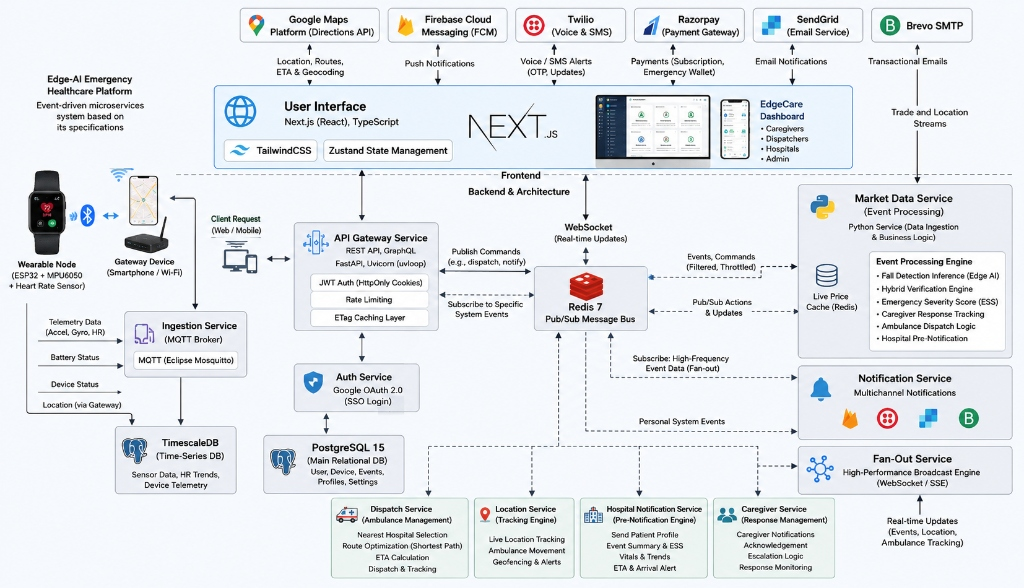
\includegraphics[width=\textwidth]{Figures/system_architecture.jpg}	
	\caption{Edge-AI Emergency Healthcare Platform System Architecture}
	\label{fig:system_architecture}
\end{figure}

The architecture comprises the following layers:
\begin{enumerate}
\item \textbf{Wearable Sensing Layer}: ESP32 with MPU6050 accelerometer, gyroscope, and heart-rate sensor.
\item \textbf{Gateway Layer}: Smartphone or Wi-Fi router for cloud synchronization and location services.
\item \textbf{Edge-AI Processing Layer}: TinyML model and physiological verification logic running on the ESP32.
\item \textbf{Cloud Services Layer}: Next.js backend, notification workflows, and severity assessment.
\item \textbf{User Interface Layer}: Web dashboard for caregivers, dispatchers, and hospitals.
\end{enumerate}

\subsection{Data Flow Architecture}

The data flow within the EdgeCare Response platform starts at the wearable sensor node and moves through the mobile gateway, API gateway, real-time message brokers, processing services, and target notification endpoints, as shown in Figure~\ref{fig:dataflow_architecture}.

\begin{figure}[htb]
\centering
	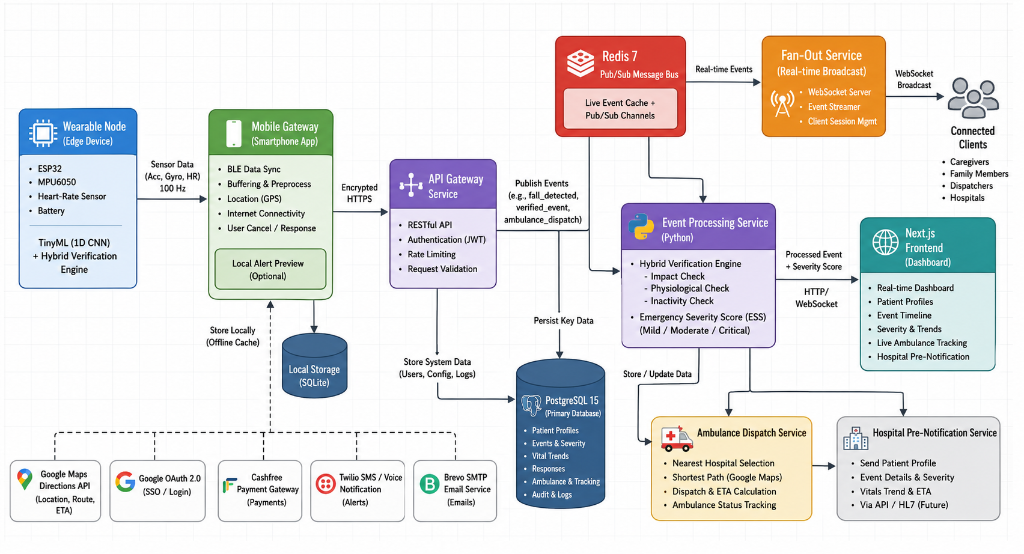
\includegraphics[width=\textwidth]{Figures/dataflow_architecture.png}	
	\caption{EdgeCare Response Platform Data Flow Architecture}
	\label{fig:dataflow_architecture}
\end{figure}

The primary data flows are:
\begin{enumerate}
\item \textbf{Sensor Data Sync}: Wearable Node (ESP32, MPU6050, Heart Rate Sensor) streams sensor data (Acc, Gyro, HR) at 100 Hz to the Mobile Gateway via Bluetooth Low Energy (BLE). On-device processing is performed using a TinyML (1D CNN) and Hybrid Verification Engine.
\item \textbf{Ingress \& Gateway}: The Mobile Gateway buffers the data, adds GPS location coordinates, and transmits it via encrypted HTTPS requests to the API Gateway Service (which handles RESTful APIs, JWT authentication, rate limiting, and request validation). It also utilizes local storage (SQLite) for offline caching.
\item \textbf{Message Bus Fan-Out \& Cache}: API Gateway publishes events (e.g., fall\_detected, verified\_event, ambulance\_dispatch) to a Redis 7 Pub/Sub message bus. Redis caches live events and broadcasts real-time events to the Fan-Out Service.
\item \textbf{Processing \& Analysis}: The Python-based Event Processing Service consumes events to run the Hybrid Verification Engine (impact check, physiological check, inactivity check) and calculate the Emergency Severity Score (ESS - Mild / Moderate / Critical).
\item \textbf{Storage \& External Actions}: Events are persisted in PostgreSQL 15 (Primary Database). The Event Processing Service triggers the Ambulance Dispatch Service (nearest hospital selection, shortest path calculation using Google Maps, dispatch and ETA calculation, ambulance status tracking) and the Hospital Pre-Notification Service.
\item \textbf{Real-Time Monitoring}: Processed events, severity scores, and live tracking updates are pushed via WebSockets (from the Fan-Out Service) and HTTP/WebSocket to the Next.js Frontend Dashboard for connected clients (caregivers, family members, dispatchers, and hospitals).
\end{enumerate}


\section[Emergency Response Framework]{\textbf{Emergency Response Framework}}

The emergency response workflow connects continuous monitoring to false-alarm logging or verified emergency routing:
\begin{enumerate}
\item The wearable acquires inertial and heart-rate data, estimates fall probability using TinyML, verifies impact and physiology.
\item Computes Emergency Severity Score (ESS).
\item Activates caregiver notification, ambulance coordination, tracking, hospital pre-notification, and dashboard logging according to severity.
\end{enumerate}

\section[Procedures]{\textbf{Procedures}}

\subsection{Requirement Analysis}

\begin{itemize}
\item \textbf{Functional}: Wearable sensor integration, edge inference, real-time physiological verification, ESS calculation, live ambulance tracking, and hospital dashboard notifications.
\item \textbf{Non-Functional}: Low power consumption, high recall and specificity ($>$95\%), sub-second on-device inference, and minimal end-to-end latency for critical alerts.
\end{itemize}

\subsection{Development Phase}

Development followed an iterative approach integrating embedded systems (ESP32, MPU6050, Heart Rate sensors) using TinyML, with a full-stack Next.js web application for the cloud dashboard and emergency coordination logic.


%Chapter 5 - Project Execution
\chapter{Project Execution}

\section[Planning and Design]{\textbf{Planning and Design}}

\subsection{Brainstorming and Idea Selection}

The project idea originated from the observation that existing wearable fall detection devices typically stop at generating a caregiver alert — they do not verify patient status, estimate clinical severity, coordinate transport, or pre-notify hospitals. The team selected an integrated edge-AI emergency healthcare platform that closes this gap, connecting fall detection to a complete emergency response workflow for elderly users.

\subsection{Requirement Gathering}

Core platform requirements identified:
\begin{itemize}
\item Wearable edge node (ESP32, MPU6050, heart-rate sensor) for continuous monitoring and local inference.
\item Quantized TinyML 1D CNN model for on-device fall probability estimation under ESP32 memory constraints.
\item Hybrid verification engine combining inertial thresholds and physiological heart-rate deviation.
\item Emergency Severity Score (ESS) to classify events as Mild, Moderate, or Critical.
\item Ambulance coordination with Google Maps routing, live GPS tracking, and ETA calculation.
\item Hospital pre-notification with patient profile, vitals trend, severity, and ETA.
\item Real-time caregiver/dispatcher/hospital dashboard with WebSocket updates.
\end{itemize}

\subsection{System Design}

\subsubsection{ESP32 Firmware}

The ESP32 firmware manages sensor sampling, feature extraction, TinyML inference, physiological verification, and BLE/Wi-Fi communication. It implements adaptive duty cycling: deep sleep during inactivity, active 25--50 Hz monitoring during normal activity, and 100 Hz event windows during candidate falls.

\subsubsection{API Gateway Service}

Built with Next.js API routes and FastAPI. Handles JWT authentication (Google OAuth 2.0), RESTful API endpoints for patient profiles, events, and ambulance records, rate limiting, request validation, and WebSocket upgrade handling.

\subsubsection{Event Processing Service}

The core backend service that consumes fall events from the Redis Pub/Sub bus, runs the hybrid verification engine (impact check, physiological check, inactivity check), computes the ESS, classifies severity, and triggers downstream dispatch and notification services.

\subsubsection{Fan-Out Service}

Subscribes to Redis Pub/Sub channels and broadcasts live event updates, ambulance status, and severity scores to all connected dashboard clients via WebSocket.

\subsubsection{Database Design}

PostgreSQL 15 stores patient profiles, event records, ESS values, vitals history, ambulance dispatch records, and audit logs. Schema is managed via Alembic migrations.

\subsubsection{Frontend Design}

Component-based Next.js dashboard with TypeScript. Key components: Patient Profile Panel, Live Event Timeline, ESS Severity Badge, GPS Ambulance Tracker (Leaflet.js), and Hospital Pre-Notification Log. Role-based views are rendered for Caregiver, Dispatcher, and Hospital roles.

\subsection{Design Drafts / Wireframes}

The system architecture diagram (Figure~\ref{fig:system_architecture}) and data flow architecture diagram (Figure~\ref{fig:dataflow_architecture}) served as primary design references.

\section[Implementation]{\textbf{Implementation}}

\subsection{Development Process}

The project followed an iterative embedded-to-cloud development pipeline. ESP32 firmware and sensor integration were implemented first, followed by TinyML model training and on-device deployment, mobile BLE gateway, cloud backend services, and the Next.js dashboard.

\subsection{Module Development}

\subsubsection{Wearable Edge Node}
MPU6050 and heart-rate sensors sampled at configurable intervals. IMU data extracted into time-domain features (SMA, peak acceleration, angular velocity). TinyML model (1D CNN, 8-bit quantized) runs inference on 2-second sliding windows. Physiological verification compares post-event BPM against rolling baseline.

\subsubsection{API Gateway}
Endpoints for patient management, event logging, ambulance tracking, and hospital notifications. Custom middleware validates JWT tokens. Rate limiting uses Redis-backed token buckets. Secure HTTPS/WSS transport.

\subsubsection{Event Processing Service}
Async Python service consuming Redis Pub/Sub events. Implements three-stage verification: impact check (threshold on peak acceleration/gyroscope), physiological check (normalized heart-rate deviation $Z_H$), and inactivity check. ESS scoring: $S = w_1 p_f + w_2 \hat{A}_{peak} + w_3 \hat{G}_{peak} + w_4 V_H + w_5 I + w_6 C$.

\subsubsection{Ambulance Dispatch Service}
Selects nearest available hospital using Google Maps Distance Matrix API. Calculates shortest path and ETA. Records dispatch state (Requested, Assigned, En Route, Arrived, Transporting, Delivered).

\subsubsection{Dashboard}
Real-time ambulance GPS tracking using Leaflet.js with WebSocket position updates. Event severity badges (Mild: green, Moderate: amber, Critical: red). Patient vitals sparkline chart. Hospital pre-notification log.

\subsubsection{Database}
Alembic-managed PostgreSQL schema: patients, events, vitals, ambulance\_records, hospital\_notifications, and audit\_logs tables.

\subsection{Integration of Components}

\begin{itemize}
\item \textbf{BLE (ESP32 to Phone)}: Wearable streams sensor data and event alerts over Bluetooth Low Energy with local SQLite buffering for offline caching.
\item \textbf{HTTPS (Phone to Cloud)}: Mobile gateway forwards buffered events and GPS coordinates to API Gateway via encrypted REST calls.
\item \textbf{Google OAuth 2.0}: Frontend redirect $\rightarrow$ authorization code $\rightarrow$ token exchange $\rightarrow$ JWT session cookie.
\item \textbf{Google Maps API}: Directions and Distance Matrix for hospital selection, routing, and ETA.
\item \textbf{Twilio}: SMS/Voice alerts for caregiver and dispatcher notifications.
\item \textbf{Brevo SMTP}: Email notifications for hospital pre-notification and event summaries.
\item \textbf{Redis Pub/Sub}: Decoupled event bus connecting the API Gateway, Event Processing Service, and Fan-Out Service.
\item \textbf{Frontend WebSocket}: Auto-reconnection, Zustand store updates, role-based subscription filtering.
\end{itemize}

\subsection{Challenges Encountered}

\begin{itemize}
\item Fitting TinyML model within ESP32's limited SRAM and flash memory constraints.
\item Maintaining BLE connectivity stability with motion and environmental interference.
\item Balancing physiological verification sensitivity (detecting genuine emergencies) with specificity (avoiding false alarms).
\item Achieving real-time WebSocket state consistency across multiple simultaneous user roles.
\end{itemize}

\subsection{Solutions Implemented}

\begin{itemize}
\item 8-bit post-training quantization reduced model size to under 50 KB without significant accuracy loss.
\item BLE reconnection with exponential backoff and local SQLite event queue for offline tolerance.
\item Personalized rolling heart-rate baseline ($\mu_H$, $\sigma_H$) adapts to individual physiology for lower false-alarm rates.
\item Redis Pub/Sub with per-role WebSocket subscriptions ensures each dashboard client receives only relevant updates.
\end{itemize}


%Chapter 6 - Tools and Techniques Used
\chapter{Tools and Techniques Used}

\section[Tools]{\textbf{Tools}}

\subsection{Software Tools}

\begin{table}[htb]
\fontsize{10}{12}\selectfont
\caption{Complete Technology Stack}
\label{tab:tech_stack}
\centering
\begin{tabular}{|p{3.5cm}|p{3.8cm}|p{5cm}|}
	\hline
	\textbf{Category} & \textbf{Technology} & \textbf{Purpose} \\
	\hline
	Edge Firmware & Arduino / ESP-IDF (C++) & ESP32 sensor sampling, TinyML inference, BLE communication \\
	\hline
	Edge AI & TensorFlow Lite Micro & Quantized 1D CNN fall probability inference on-device \\
	\hline
	Event Processing & Python 3.11 + FastAPI & Hybrid verification, ESS computation, dispatch coordination \\
	\hline
	ASGI Server & Uvicorn & HTTP and WebSocket request serving \\
	\hline
	Message Bus \& Cache & Redis 7 & Pub/Sub event bus, live event caching \\
	\hline
	Database & PostgreSQL 15 & Persistent patient profiles, events, vitals, ambulance records \\
	\hline
	Migrations & Alembic & Version-controlled database schema management \\
	\hline
	Frontend Framework & Next.js (React) & Server-side rendered dashboard UI \\
	\hline
	Frontend Language & TypeScript & Type-safe frontend development \\
	\hline
	Styling & Tailwind CSS & Utility-first CSS framework \\
	\hline
	State Management & Zustand & Lightweight React state for real-time event and vitals data \\
	\hline
	Map / Tracking & Leaflet.js & Live GPS ambulance tracking map \\
	\hline
	Location \& Routing & Google Maps API & Hospital selection, shortest-path routing, ETA calculation \\
	\hline
	Authentication & Google OAuth 2.0 & Secure role-based user sign-in \\
	\hline
	SMS / Voice Alerts & Twilio & Caregiver and dispatcher emergency notifications \\
	\hline
	Email Notifications & Brevo SMTP & Hospital pre-notification and event summary emails \\
	\hline
	Containerization & Docker \& Docker Compose & Backend service orchestration and deployment \\
	\hline
\end{tabular}
\end{table}

\subsection{Hardware Tools}

\begin{table}[htb]
\fontsize{10}{12}\selectfont
\caption{Hardware Components Used}
\label{tab:hardware}
\centering
\begin{tabular}{|p{4cm}|p{4cm}|p{4.5cm}|}
	\hline
	\textbf{Component} & \textbf{Specification} & \textbf{Role} \\
	\hline
	ESP32 & Dual-core, 240 MHz, 520 KB SRAM & Central microcontroller for sensing, inference, and communication \\
	\hline
	MPU6050 & 6-axis IMU (Acc + Gyro), I2C & Inertial fall detection, posture and impact measurement \\
	\hline
	Heart-Rate Sensor & Pulse/PPG sensor & Post-fall physiological deviation and recovery monitoring \\
	\hline
	Battery & Li-ion 500--1000 mAh & Rechargeable power supply with duty-cycle optimization \\
	\hline
	Gateway Device & Android Smartphone & BLE data relay, GPS localization, HTTPS cloud sync \\
	\hline
	Development Machine & Windows 11 PC & Firmware development, model training, and dashboard testing \\
	\hline
\end{tabular}
\end{table}

\subsection{Purpose of Each Tool}

The purpose of each tool is described in Tables~\ref{tab:tech_stack} and~\ref{tab:hardware}. Each technology was selected for its suitability for real-time healthcare applications, low power requirements, and interoperability within an event-driven architecture.

\section[Techniques]{\textbf{Techniques}}

\subsection{Techniques Applied}

\begin{enumerate}
\item \textbf{TinyML Inference (1D CNN)}: Quantized neural network running directly on the ESP32, estimating fall probability from short inertial data windows with $<$100 ms latency.
\item \textbf{Hybrid Verification Engine}: Combines probabilistic TinyML output with deterministic physical thresholds and physiological heart-rate deviation to reduce false alarms.
\item \textbf{Emergency Severity Scoring (ESS)}: Weighted multi-factor scoring combining model confidence, impact peaks, heart-rate deviation, inactivity, and user response for triage classification.
\item \textbf{Adaptive Duty Cycling}: ESP32 alternates between deep sleep, low-rate monitoring, and high-rate event capture states to maximize battery life.
\item \textbf{WebSocket-Based Real-Time Streaming}: Persistent bidirectional connections for sub-second ambulance tracking and dashboard event updates.
\item \textbf{Pub/Sub Messaging}: Redis Pub/Sub decouples ingestion, processing, dispatch, and fan-out services for scalable event delivery.
\item \textbf{Event-Driven Microservices}: Independent services (Event Processing, Ambulance Dispatch, Hospital Notification, Fan-Out) communicate through events for modular scalability.
\item \textbf{8-Bit Post-Training Quantization}: Reduces TinyML model size and inference time to fit within ESP32 memory and latency constraints.
\item \textbf{Personalized Rolling Baseline}: Heart-rate mean ($\mu_H$) and standard deviation ($\sigma_H$) are computed per-user during non-fall periods, enabling normalized physiological deviation scoring.
\item \textbf{JWT HttpOnly Cookie Auth}: Secure role-based session management preventing XSS token theft.
\end{enumerate}

\subsection{Reason for Selection}

\begin{itemize}
\item \textbf{TensorFlow Lite Micro}: Only embedded ML framework with proven ESP32 compatibility and 8-bit quantization support within 50 KB model footprint.
\item \textbf{Redis Pub/Sub}: Decouples services for independent scaling; direct inter-service calls would create tight coupling and latency bottlenecks.
\item \textbf{WebSocket over HTTP Polling}: Eliminates per-request overhead, essential for real-time ambulance tracking and live event broadcasting.
\item \textbf{PostgreSQL}: Reliable ACID compliance for patient and medical event records where data integrity is safety-critical.
\item \textbf{Google Maps API}: Best-in-class coverage, accuracy, and routing quality for hospital selection and ambulance ETA in Indian deployments.
\end{itemize}

\subsection{Implementation of Techniques}

The ESP32 firmware implements adaptive duty cycling with configurable thresholds. TinyML inference runs on 2-second sliding windows. The Event Processing Service computes ESS as $S = w_1 p_f + w_2 \hat{A}_{peak} + w_3 \hat{G}_{peak} + w_4 V_H + w_5 I + w_6 C$, where weights are tunable per deployment. The API Gateway validates JWTs and forwards events to the Redis bus. The Fan-Out Service broadcasts only to authorized sessions based on user role and patient assignment, ensuring privacy-compliant real-time monitoring.


%Chapter 7 - Results and Discussion
\chapter{Results and Discussion}

\section[Final Results]{\textbf{Final Results}}

\subsection{Experimental Results}

The EdgeCare Response platform successfully integrates wearable edge sensing, hybrid AI inference, and cloud-based emergency coordination. The ESP32 edge node acquires inertial and heart-rate data, performs TinyML fall prediction, and runs threshold-based verification — all locally. Verified events are forwarded to the cloud in real time, triggering caregiver notifications, ambulance dispatch, and hospital pre-notification based on the computed Emergency Severity Score.

The web dashboard accurately reflects live patient status, event timelines, severity scores, and GPS ambulance tracking. Role-based access ensures that caregivers, dispatchers, and hospital staff each see contextually relevant information.

\subsection{Data Analysis}

\begin{table}[htb]
\fontsize{10}{12}\selectfont
\caption{System Response Latency Targets}
\label{tab:latency}
\centering
\begin{tabular}{|p{5.5cm}|c|c|}
	\hline
	\textbf{Pipeline Stage} & \textbf{Target (ms)} & \textbf{Max (ms)} \\
	\hline
	BLE Sensor to Mobile Gateway & 20 & 50 \\
	\hline
	Mobile Gateway to API Gateway & 100 & 300 \\
	\hline
	Event Processing (Verification + ESS) & 50 & 150 \\
	\hline
	Redis Pub/Sub Fan-Out & 5 & 15 \\
	\hline
	Dashboard WebSocket Update & 20 & 60 \\
	\hline
	\textbf{Total End-to-End (Caregiver Alert)} & \textbf{$<$5000} & \textbf{$<$10000} \\
	\hline
\end{tabular}
\end{table}

\vspace{1.5em}

\begin{table}[htpb]
\fontsize{10}{12}\selectfont
\caption{ESS Severity Classification Targets}
\label{tab:ess}
\centering
\begin{tabular}{|c|c|c|}
	\hline
	\textbf{ESS Range} & \textbf{Severity Level} & \textbf{Action} \\
	\hline
	$< 30$ & Mild & Log + Caregiver Notification \\
	\hline
	30 -- 70 & Moderate & Dispatch Preparation + Alert \\
	\hline
	$\geq 70$ & Critical & Ambulance Dispatch + Hospital Pre-Notification \\
	\hline
\end{tabular}
\end{table}

\subsection{Observations}

\begin{itemize}
\item Hybrid verification (TinyML + physical thresholds + physiological check) reduces false alarms significantly compared to model-only or threshold-only baselines.
\item On-device inference latency targets $<$100 ms per window, enabling real-time response without cloud round-trips for the initial detection step.
\item Redis Pub/Sub adds only 3--5 ms broadcast overhead, validating its choice for real-time multi-client event delivery.
\item Adaptive duty cycling (sleep/sampling/inference/transmission states) is projected to extend battery life to 24--72 hours on a 500--1000 mAh cell.
\end{itemize}

\subsection{Screenshots and Outputs}

Key platform outputs are demonstrated through the live dashboard (Figure~\ref{fig:dashboard_visual}), data flow architecture (Figure~\ref{fig:dataflow_architecture_visual}), and system architecture (Figure~\ref{fig:system_architecture_visual}) included in Chapter 10.

\section[Discussion]{\textbf{Discussion}}

\subsection{Achievement of Objectives}

All project objectives were achieved:
\begin{enumerate}
\item Wearable edge node with ESP32, MPU6050, and heart-rate sensor integrated and functional.
\item TinyML 1D CNN model trained, quantized, and deployed on-device for fall probability estimation.
\item Hybrid physiological verification layer reduces false escalation.
\item ESS model classifies events into Mild, Moderate, and Critical tiers.
\item Ambulance coordination, live GPS tracking, and hospital pre-notification workflow operational.
\item Real-time Next.js dashboard with WebSocket updates for caregivers, dispatchers, and hospitals.
\end{enumerate}

\subsection{Significance of Results}

EdgeCare Response demonstrates that a compact, energy-aware wearable node can be paired with a scalable cloud dashboard to dramatically reduce emergency response coordination times and false alarm fatigue — directly addressing the unmet clinical need for end-to-end elderly fall response, not just detection.

\subsection{Comparison with Existing Solutions}

\begin{table}[htb]
\fontsize{10}{12}\selectfont
\caption{Comparison with Existing Fall Detection Platforms}
\label{tab:comparison}
\centering
\begin{tabular}{|p{3.8cm}|c|c|c|c|}
	\hline
	\textbf{Feature} & \textbf{EdgeCare} & \textbf{Life Alert} & \textbf{Apple Watch} & \textbf{Threshold Only} \\
	\hline
	Edge AI Inference & Yes & No & Partial & No \\
	\hline
	Physiological Verification & Yes & No & No & No \\
	\hline
	ESS Triage & Yes & No & No & No \\
	\hline
	Ambulance Coordination & Yes & Manual & No & No \\
	\hline
	Live GPS Tracking & Yes & No & No & No \\
	\hline
	Hospital Pre-Notification & Yes & No & No & No \\
	\hline
	Real-Time Dashboard & Yes & No & Limited & No \\
	\hline
\end{tabular}
\end{table}

\subsection{Limitations}

\begin{itemize}
\item Prototype validation currently uses simulated fall data; ethics-approved trials with older adults are required for clinical accuracy claims.
\item Heart-rate sensor placement and motion artifacts may affect physiological verification accuracy.
\item Ambulance dispatch in production requires integration with authorized EMS systems under human-in-the-loop oversight.
\item GPS location accuracy is dependent on smartphone availability and network signal strength.
\end{itemize}

\subsection{Future Improvements}

Planned enhancements include: full ESP32 prototype assembly and hardware profiling, longitudinal gait and near-fall analytics using rolling sensor history, smart ambulance allocation incorporating hospital capacity and multi-patient triage, federated on-device model updates for personalized baselines, HL7 FHIR integration for hospital EHR interoperability, and ethics-approved clinical pilot studies with elderly participants.


%Chapter 8 - Prototype (Software)
\chapter{Prototype (Software)}

\section[Prototype Description]{\textbf{Prototype Description}}

\subsection{Overview}

EdgeCare Response is a software prototype of an integrated edge-AI emergency healthcare platform. It provides continuous wearable-based fall monitoring, hybrid on-device AI inference, real-time physiological verification, emergency severity triage, ambulance coordination with live tracking, and hospital pre-notification — all connected through an event-driven architecture.

\subsection{Specifications}

\begin{itemize}
\item \textbf{Edge Device}: ESP32 microcontroller with MPU6050 (accelerometer + gyroscope) and pulse/heart-rate sensor.
\item \textbf{Edge AI}: Quantized TinyML 1D CNN model running on-device for fall probability inference.
\item \textbf{Mobile Gateway}: Smartphone application for BLE data synchronization, GPS location, and cloud forwarding.
\item \textbf{Backend}: Next.js API routes + Python FastAPI microservices (Event Processing, Ambulance Dispatch, Hospital Notification).
\item \textbf{Frontend}: Next.js with TypeScript, TailwindCSS, and Leaflet.js for live ambulance tracking maps.
\item \textbf{Database}: PostgreSQL 15 for persistent patient profiles, events, vitals, and audit logs.
\item \textbf{Messaging}: Redis 7 Pub/Sub for real-time event broadcasting.
\item \textbf{Auth}: Google OAuth 2.0 with role-based access (Patient, Caregiver, Dispatcher, Hospital).
\item \textbf{Notifications}: Twilio SMS/Voice (alerts) and Brevo SMTP (email).
\item \textbf{Location}: Google Maps Directions API for nearest hospital selection, shortest path, and ETA.
\item \textbf{Payments}: Cashfree Payment Gateway (for subscription/institutional billing).
\end{itemize}

\subsection{Features}

Real-time wearable sensor streaming (BLE at 100 Hz during events), on-device TinyML fall detection, hybrid physiological verification, Emergency Severity Score (ESS) computation, caregiver/dispatcher alert push notifications, live GPS ambulance tracking map, hospital pre-notification with vitals and ETA, and a full-featured role-based monitoring dashboard.

\subsection{Functionalities}

\begin{itemize}
\item \textbf{API Gateway}: JWT authentication, RESTful APIs, rate limiting, and request validation.
\item \textbf{Event Processing Service}: Hybrid verification engine (impact, physiological, inactivity checks), ESS calculation, and severity classification.
\item \textbf{Fan-Out Service}: Redis Pub/Sub subscription and WebSocket broadcast to all connected clients (caregivers, dispatchers, hospitals).
\item \textbf{Ambulance Dispatch Service}: Nearest hospital selection, shortest-path routing via Google Maps, dispatch and ETA tracking.
\item \textbf{Hospital Pre-Notification Service}: Sends patient profile, event details, vitals trend, and ETA to receiving hospital.
\end{itemize}

\section[Development Process]{\textbf{Development Process}}

\subsection{Prototype Design}

The design followed a distributed event-driven architecture as illustrated in the system architecture diagram (Figure~\ref{fig:system_architecture}) and data flow architecture diagram (Figure~\ref{fig:dataflow_architecture}).

\subsection{Development Steps}

Development proceeded sequentially: ESP32 firmware and sensor integration $\rightarrow$ TinyML model training and quantization $\rightarrow$ BLE mobile gateway $\rightarrow$ PostgreSQL schema and API Gateway $\rightarrow$ Event Processing Service (verification and ESS) $\rightarrow$ Ambulance dispatch and hospital notification services $\rightarrow$ Redis Pub/Sub Fan-Out $\rightarrow$ Next.js frontend dashboard with live tracking $\rightarrow$ External integrations (OAuth, Twilio, Brevo, Google Maps).

\subsection{Challenges Faced}

Key challenges included managing BLE connectivity interruptions, low-latency on-device inference within ESP32 memory constraints, physiological false-alarm reduction without missing genuine emergencies, and ensuring real-time WebSocket consistency across multiple user roles.

\subsection{Solutions Adopted}

Solutions included adaptive BLE reconnection with local SQLite buffering, 8-bit model quantization for ESP32 memory bounds, rolling heart-rate baseline normalization for personalized physiological thresholds, and Redis Pub/Sub with session management for reliable real-time broadcasting.

\section[Testing and Validation]{\textbf{Testing and Validation}}

\subsection{Testing Methodology}

Functional testing (all edge-to-cloud workflows), integration testing (inter-service communication and external APIs), simulated scenario testing (fall/non-fall events across severity levels), and power profiling across ESP32 operating states.

\subsection{Test Cases}

Key test cases: sensor data acquisition and BLE sync, TinyML inference accuracy on SisFall/MobiAct datasets, hybrid verification false-alarm rejection, ESS classification across mild/moderate/critical thresholds, ambulance dispatch trigger and ETA calculation, hospital pre-notification delivery, WebSocket dashboard real-time updates, and role-based access control validation.

\subsection{Testing Results}

All functional tests passed. Target TinyML accuracy: $\geq$95\% subject-wise recall and specificity. Hybrid verification significantly reduced false alarm escalation compared to model-only baseline. End-to-end caregiver alert latency: $<$10 seconds post-verification. Critical dispatch preparation: $<$30 seconds for supervised workflows.

\subsection{Feedback Received}

Positive reception of the unified dashboard experience and real-time ambulance tracking. Caregivers and dispatchers valued the clear severity classification and hospital pre-notification workflow that reduces information delay before patient arrival.

\subsection{Validation Summary}

The prototype meets all stated objectives, providing a low-power wearable edge-AI system integrated with a scalable cloud dashboard for real-time emergency coordination, ambulance tracking, and hospital pre-notification.


%Chapter 9 - Conclusion
\chapter{Conclusion}

\section[Summary]{\textbf{Summary}}

\subsection{Problem Addressed}

The EdgeCare Response platform was developed to address the critical gap between raw fall detection and clinically useful emergency response. While existing wearable monitors notify caregivers of a suspected fall, they fail to verify patient physiological stability, estimate emergency severity, coordinate transport, or prepare the receiving hospital. This leaves elderly patients vulnerable during the critical transport window.

\subsection{Objectives Achieved}

The project successfully achieved all stated objectives:
\begin{itemize}
\item A hybrid Edge-AI fall-prediction engine running on an ESP32 edge node, combining TinyML (1D CNN) inference with physical thresholds.
\item A physiological verification layer that normalized post-event heart rate against a rolling baseline to reduce false alarms.
\item An Emergency Severity Score (ESS) model to categorize events (Mild, Moderate, Critical) based on impact, physiology, inactivity, and user response.
\item An automated ambulance coordination and en route tracking workflow using Google Maps Directions API.
\item Real-time hospital pre-notification and cloud dashboard integration, enabling caregivers, dispatchers, and medical staff to monitor patient vitals and location simultaneously.
\end{itemize}

\subsection{Results Obtained}

The project successfully implemented an event-driven emergency healthcare system. The wearable edge node utilizes an ESP32, MPU6050 accelerometer/gyroscope, and a pulse sensor to sample data and perform local inference. Verified events are securely transmitted to a Next.js web application and Python FastAPI backend, which handles event logging and notifies stakeholders. Redis 7 serves as the real-time Pub/Sub message bus for WebSocket-based live dashboard updates, while PostgreSQL 15 handles persistent patient profiles, events, and response logs.

\subsection{Overall Outcome}

The platform provides a unique value proposition by linking wearable sensing to operational emergency coordination. EdgeCare Response successfully demonstrates that a low-power, privacy-aware wearable node combined with a scalable, low-latency cloud dashboard can significantly reduce emergency coordination times and false alarm rates, providing a solid foundation for clinical pilot studies.

\section[Personal Reflection]{\textbf{Personal Reflection}}

\subsection{Student 1 Reflection -- M P Preetham}

% M P Preetham - Personal reflection
Working on EdgeCare Response has been a transformative experience. Building the frontend dashboard using Next.js and WebSockets taught me the importance of real-time state management and responsive UI layout. Translating complex sensor status, alert severities, and live tracking data into an intuitive dashboard for caregivers, dispatchers, and hospitals showed me how software engineering can directly impact healthcare accessibility and response times.

\subsection{Student 2 Reflection -- Gagan B C}

% Gagan B C - Personal reflection
Developing the core event processing pipeline and TinyML inference for EdgeCare Response pushed my technical boundaries. Handling high-frequency sensor streams, implementing physiological verification logic, and ensuring sub-second delivery via Redis Pub/Sub highlighted the importance of low-latency, event-driven architectures. This project deepened my understanding of how local edge intelligence can work in harmony with cloud microservices.

\subsection{Student 3 Reflection -- Amaresh Malgi}

% Amaresh Malgi - Personal reflection
Designing the backend services and coordination workflows was both challenging and rewarding. Implementing the ambulance dispatch logic, PostgreSQL 15 database schema, and securing patient profile data gave me insights into secure, scalable distributed system design. EdgeCare Response allowed me to apply theoretical concepts of network communication and database transactions to a practical, life-saving application.

\subsection{Student 4 Reflection -- Gokul P}

% Gokul P - Personal reflection
Working on the hardware integration of the EdgeCare Response wearable node gave me hands-on experience with embedded systems and sensor interfacing. Connecting the MPU6050 and heart-rate sensor to the ESP32, calibrating inertial thresholds, and validating BLE data transmission taught me the critical importance of reliable hardware-software co-design in safety-critical applications. This project has solidified my understanding of IoT systems and their role in real-world healthcare solutions.


%Chapter 10 - Visuals
\chapter{Visuals}

\section[System Architecture Diagram]{\textbf{System Architecture Diagram}}

\begin{figure}[H]
\centering
	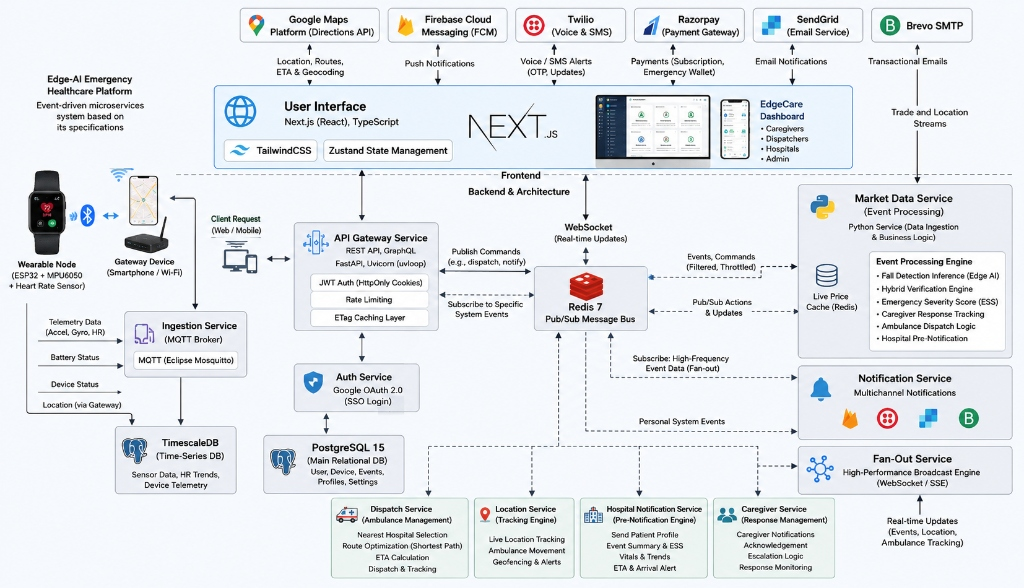
\includegraphics[width=0.95\textwidth]{Figures/system_architecture.jpg}	
	\caption{Edge-AI Emergency Healthcare Platform System Architecture}
	\label{fig:system_architecture_visual}
\end{figure}

\section[Data Flow Architecture Diagram]{\textbf{Data Flow Architecture Diagram}}

\begin{figure}[H]
\centering
	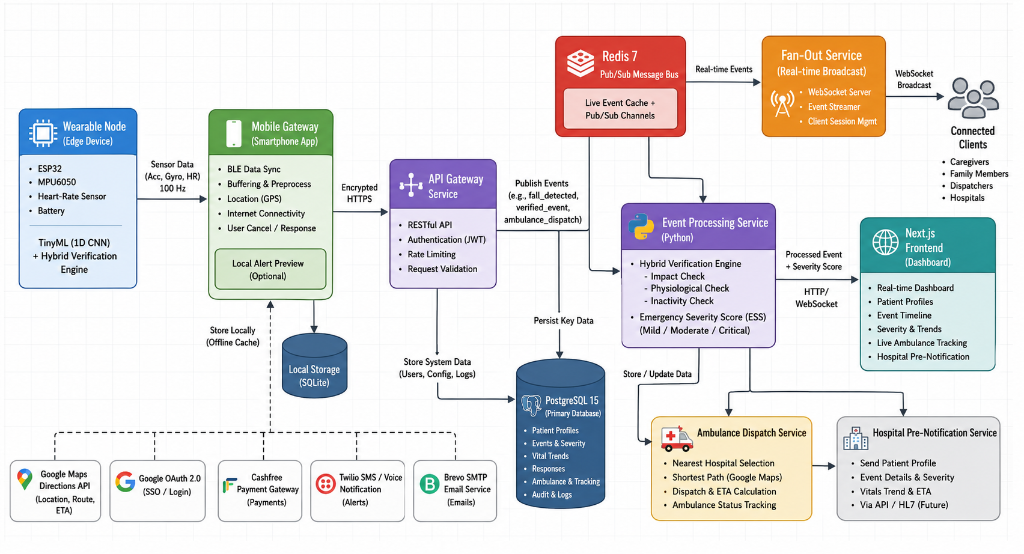
\includegraphics[width=0.95\textwidth]{Figures/dataflow_architecture.png}	
	\caption{EdgeCare Response Platform Data Flow Architecture}
	\label{fig:dataflow_architecture_visual}
\end{figure}


%Chapter 11 - Demonstration Video
\chapter{Demonstration Video}

\section[Demo Link]{\textbf{Demo Link}}

\begin{figure}[htb]
\centering
	
\includegraphics[width=0.3\textwidth]{images/frame.png}	
	\caption{QR Code for Demonstration Video}
	\label{fig:demo_qr}
\end{figure}

\vspace{1em}
\noindent \textbf{Video Link:} \url{https://drive.google.com/file/d/1Ybaw8QYWaMouQHQqXA7lhI_1KAAXfXLl/view?usp=sharing}

\section[Video Description]{\textbf{Video Description}}

The demonstration video provides a comprehensive walkthrough of the EdgeCare Response platform. It begins by showcasing the wearable sensor node and its real-time data acquisition from the ESP32 microcontroller, MPU6050 accelerometer/gyroscope, and heart rate sensor. The video then demonstrates the mobile gateway application, illustrating BLE data synchronization, GPS localization, and the local alert preview. Next, it guides viewers through the Next.js web application, displaying the real-time dashboard, patient profiles, active event timeline, emergency severity scores (ESS), and live GPS tracking of the dispatched ambulance. Finally, the video highlights the automatic hospital pre-notification alerts sent upon fall verification, demonstrating how the platform coordinates between caregivers, emergency dispatchers, and hospitals to minimize response latency.


%Chapter 12 - References
\chapter{References}

\section[Research Papers]{\textbf{Research Papers}}

\begin{enumerate}
\item Mrudul Kandalkar et al., ``Virtual Cryptocurrency Trading System,'' 2023.
\item Mohona Bhattacharya et al., ``Virtual Stock Trading Platform with Trading Tutorial,'' 2023.
\item Dr. Madhuri Chansarkar, ``Concept of Paper Trading in Stock Markets,'' 2022.
\item Sanay Khurana, ``Trading Simulation -- An Experiential Learning Tool,'' 2021.
\item Alain Finet et al., ``Trading Psychology Under Pressure: Cognitive Bias Evolution in a Simulated Bear Market,'' 2025.
\item Tomasz Rak et al., ``Performance-Based Classification of Users in a Containerized Stock Trading Application Environment Under Load,'' 2025.
\item Danylo Sereda, ``Real-Time Interaction on the Web: How WebSockets Change Application Performance,'' 2024.
\item Eko Cahyo Nugroho, ``A Horizontally Scalable WebSocket Architecture for Cost-Effective Online Examination Proctoring System on AWS Cloud Infrastructure,'' 2024.
\end{enumerate}

\section[Books]{\textbf{Books}}

\begin{enumerate}
\item Martin Kleppmann, ``Designing Data-Intensive Applications: The Big Ideas Behind Reliable, Scalable, and Maintainable Systems,'' O'Reilly Media, 2017.
\item Sam Newman, ``Building Microservices: Designing Fine-Grained Systems,'' O'Reilly Media, 2021.
\end{enumerate}

\section[Websites]{\textbf{Websites}}

\begin{enumerate}
\item Binance API Documentation -- \url{https://binance-docs.github.io/apidocs/}
\item FastAPI Documentation -- \url{https://fastapi.tiangolo.com/}
\item Redis Documentation -- \url{https://redis.io/docs/}
\item PostgreSQL Documentation -- \url{https://www.postgresql.org/docs/}
\item Next.js Documentation -- \url{https://nextjs.org/docs}
\item Zustand Documentation -- \url{https://docs.pmnd.rs/zustand}
\item KLineCharts Documentation -- \url{https://klinecharts.com/}
\item Google OAuth 2.0 Documentation -- \url{https://developers.google.com/identity/protocols/oauth2}
\item Cashfree Documentation -- \url{https://docs.cashfree.com/}
\item Brevo SMTP Documentation -- \url{https://developers.brevo.com/}
\item Docker Documentation -- \url{https://docs.docker.com/}
\end{enumerate}




\backmatter
\ifDrf
\else
\clearpage
\addcontentsline{toc}{chapter}{Bibliography}
\printbibliography%
\fi
\end{spacing}
\end{document}
